\newpage
\subsection{Goal}\label{subsec:goal}

The use of stochastic and metaheuristic algorithms (Simulated Annealing, Differential Evolution, Particle Swarm Optimization) in the tasks of unconstrained nonlinear optimization and the experimental comparison of them with Nelder-Mead and Levenberg-Marquardt algorithms.

\subsection{Formulation of the problem}\label{subsec:formulation-of-the-problem}

Generate the noisy data $(x_k, y_k)$, where $k = 0, \dots, 1000$, according to the rule:

\begin{equation*}
y = \begin{cases}
-100 + \delta_k, & f(x_k) < -100, \\
f(x_k) + \delta_k & -100 \leq f(x_k) \leq 100, \\
100 + \delta_k & f(x_k) > 100,
\end{cases}
\end{equation*}

\begin{equation*}
    x_k = \frac{3k}{1000},
\end{equation*}

\begin{equation*}
    f(x) = \frac{1}{x^2 - 3x + 2},
\end{equation*}

where $\delta_x \approx N(0, 1)$ are values of a random variable with standard normal distribution.
Approximate the data by the rational function

\begin{equation*}
    F(x, a, b, c, d) = \frac{ax + b}{x^2 + cx + d},
\end{equation*}

by means of least squares through the numerical minimization of the following function:

\begin{equation*}
    D(a, b, c, d) = \sum^{1000}_{k=0}(F(x_k, a, b, c, d) - y_k)^2.
\end{equation*}

To solve the minimization problem, use Nelder-Mead algorithm, Levenberg-Marquardt algorithm and at least two of the methods among Simulated Annealing, Differential Evolution and Particle Swarm Optimization.
If necessary, set the initial approximations and other parameters of the methods.
Use $\varepsilon = 0.001$ as the precision;
at most 1000 iterations are allowed.
Visualize the data and the approximants obtained in a single plot.
Analyze and compare the results obtained (in terms of number of iterations, precision, number of function evaluations, etc.).

\subsection{Brief theoretical part}\label{subsec:brief-theoretical-part}

Optimization methods are numerical methods for finding optimal (in some sense) values of objective functions, for example, in the framework of mathematical models of certain processes.

\textit{Stochastic algorithms} are a broad class of algorithms that rely on repeated random sampling to solve an optimization problem.
These methods are useful when it is impossible or difficult to apply others.

\textit{Metaheuristic algorithms} are algorithms inspired by natural phenomena that solve the optimization problem by trial and error.
Metaheuristic methods do not guarantee that a solution to the optimization problem will be found.

\paragraph{Nelder-Mead.}

If the function $f(x)$ is a ravine function, the efficiency of the simplex method in solving problem:
\begin{equation*}
    \min_{x \in R^n} f(x) = f(x*) = f*
\end{equation*}
is significantly reduced due to the fact that the regular simplex cannot be "extended" along the ravine.
The Nelder-Mead method (the deformable polyhedron method) is a development of the simplex method and uses the deformation of the current simplex (not necessarily regular) in the search process.
The method uses the following operations on simplexes:

\begin{itemize}
    \item reflection;
    \item reduction;
    \item compression;
    \item stretching.
\end{itemize}

\paragraph{Levenberg-Marquardt algorithm}

The \textit{Levenberg-Marquardt algorithm} (\textit{LMA}) is a popular trust region algorithm that is used to find a minimum of a function (either linear or nonlinear) over a space of parameters.
Essentially, a trusted region of the objective function is internally modeled with some function such as a quadratic.
When an adequate fit is found, the trust region is expanded.
As with many numerical techniques, the Levenberg-Marquardt method can be sensitive to the initial starting parameters.

\paragraph{Simulated annealing}
\textit{Simulated annealing} is a random-search technique which exploits an analogy between the way in  which a metal cools and freezes into a minimum energy crystalline structure (the annealing process) and  the search for a minimum in a more general system;
it forms the basis of an optimisation technique for combinatorial and other problems.

\paragraph{Differential evolution}
\textit{Differential evolution} is one of the most influential optimization algorithms up-to-date.
Differential evolution works through analogous computational steps as used by a standard evolutionary algorithm.

\subsection{Results}\label{subsec:results}

In the case of a \textit{rational approximation}, significant nonlinearities occur, so the result depends on the initial approximations (Figure~\ref{ris:plot}).

\begin{figure}[H]
    \center
    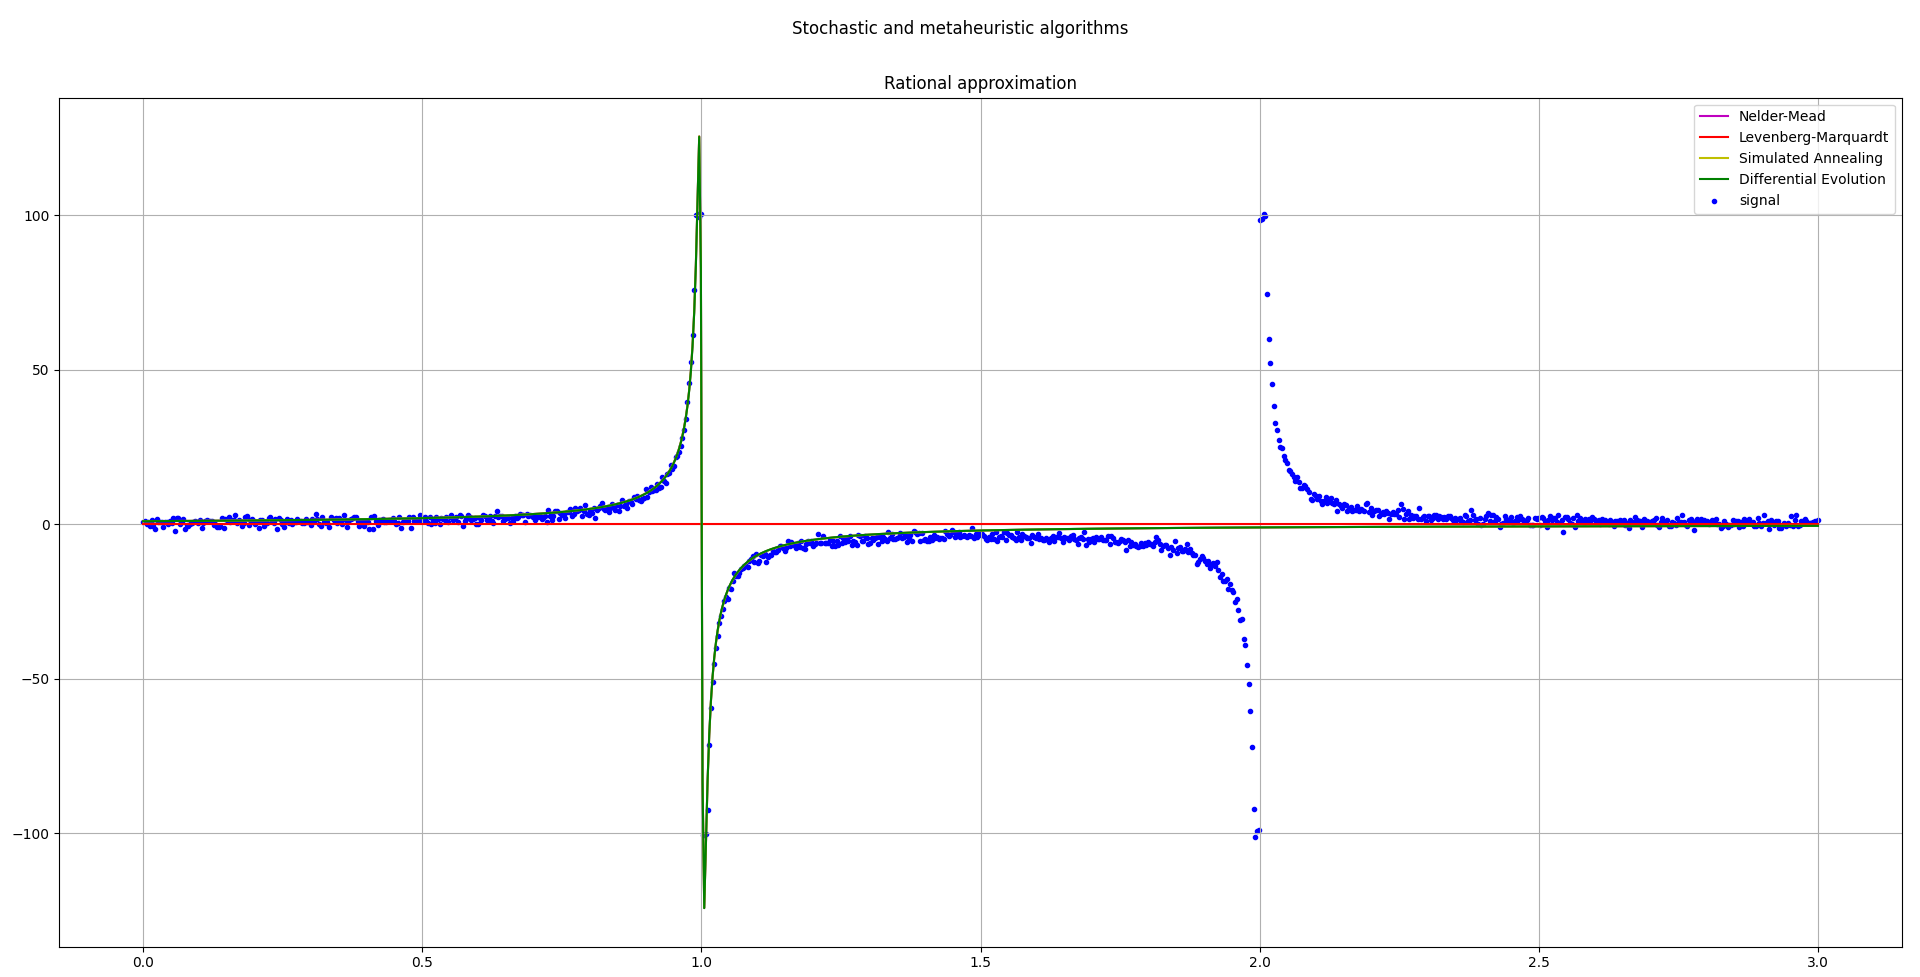
\includegraphics[width=\textwidth]{img/plot.png}
    \caption{Stochastic and metaheuristic algorithms.}
    \label{ris:plot}
\end{figure}

From the table below (Table,~\ref{tbl:stohmeta}) it is evident that methods \textit{Nelder-Mead} and \textit{Levenberg-Marquardt} require an order of magnitude less number of computations.
However, despite the fact that metaheuristic methods do not guarantee finding the result, they allow you to get a solution of fairly good quality in an acceptable time without knowing the search space.

Note that both metaheuristic methods produced extremely similar results for different numbers of iterations.

\begin{table}[ht]
\caption{Stochastic and metaheuristic algorithms}
\begin{tabular}{l|l|c|c|}
\cline{2-4}
                                                         & \textbf{method}                 & \multicolumn{1}{l|}{\textbf{iterations}} & \multicolumn{1}{l|}{\textbf{function eval}} \\ \hline
\multicolumn{1}{|l|}{\multirow{4}{*}{\textbf{rational}}} & \textit{Nelder-Mead}            & 480                                      & 795                                         \\ \cline{2-4}
\multicolumn{1}{|l|}{}                                   & \textit{Levenberg-Marquardt}    & nan                                      & 3                                           \\ \cline{2-4}
\multicolumn{1}{|l|}{}                                   & \textit{Simulated Annealing}    & 1000                                     & 9111                                        \\ \cline{2-4}
\multicolumn{1}{|l|}{}                                   & \textit{Differential Evolution} & 149                                      & 9105                                        \\ \hline
\end{tabular}
\label{tbl:stohmeta}
\end{table}

\subsection{Conclusion}\label{subsec:conclusion}

In the course of the laboratory work, stochastic and metaheuristic algorithms were implemented and analyzed within the problem of the unconstrained optimization problem.
This paper also provides a comparative analysis of stochastic and metaheuristic algorithms.

\subsection{Appendix}\label{subsec:appendix}

The source code is located \href{https://github.com/vanSultan/anal_dev_algo/tree/lab_04}{here}: \url{https://github.com/vanSultan/anal_dev_algo/tree/lab_04}.
